\newpage
\section{Алгоритм решения задачи и его анализ}

\subsection{Идея алгоритма}
Одним из наиболее известных конструктивных алгоритмов для решения поставленной задачи является жадный алгоритм $\sf{LPT}$ (Longest-processing-time-first scheduling). Другими популярными алгоритмами аппроксимации поставленной задачи являются $\sf{List}$ $\sf{scheduling}$, $\sf{MULTIFIT}$, $\sf{COMBINE}$ и $\sf{LISTFIT}$. Последние три теоретически дают наиболее точную аппроксимацию, но требуют больше вычислительных ресурсов (подробнее про их коэффициент аппроксимации и временную сложность см. в [3]). В то же время на практике алгоритм $\sf{LPT}$ работает лучше и, кроме того, он прост в реализации.

\subsection{Правило $\sf{LPT}$}
Алгоритм $\sf{LPT}$ работает следующим образом:
\begin{enumerate}
    \item Сначала он сортирует работы в порядке убывания времени их выполнения;
    \item Далее он назначает работы одну за другой в таком порядке, чтобы очередная работа планировалась на машину с наименьшей в данный момент нагрузкой. 
\end{enumerate}
Второй шаг алгоритма по сути является алгоритмом $\sf{List}$ $\sf{scheduling}$. Разница в том, что последний перебирает задачи в произвольном порядке, в то время как $\sf{LPT}$ предварительно упорядочивает их по времени обработки.

\subsection{Коэффициент аппроксимации}
$\sf{LPT}$ был впервые проанализирован Рональдом Грэмом в 1960-х годах в контексте проблемы о назначении задач. Докажем, что достигается $\frac{4}{3}$-приближение. Идею достаточно простого и прямого доказательства автор статьи нашёл в документе [3].  

Обозначим через $OPT$ время выполнения в случае оптимального назначения работ для $P||C_{max}$. Разделим множество данных работ $J$ на три группы: 
\begin{enumerate}
    \item Простые, $p_{i} \leq \frac{1}{3}OPT$
    \item Средние, $\frac{1}{3}OPT < p_{i} \leq \frac{2}{3}OPT$
    \item Тяжёлые, $\frac{2}{3}OPT < p_{i}$
\end{enumerate}

\noindent
Выделим три этапа работы алгоритма $\sf{LPT}$:
\begin{enumerate}
    \item Сначала $m$ самых длинных работ назначаются на машины. В случае, если $|n| \leq |m|$, алгоритм завершает свою работу
    \item Далее алгоритм продолжает назначать задачи, пока очередной выбранной машиной (с наименьшей в данный момент нагрузкой) не станет та, которая выполнила уже две назначенные работы, или пока все задачи не будут назначены
    \item Далее алгоритм распределяет оставшиеся задачи, пока все из них не будут назначены
\end{enumerate}

\noindent
Обозначим значения целевой функции после каждого из описанных выше этапов через $C_{max}^{1}$, $C_{max}^{2}$ и $C_{max}^{3}$ соответственно. Заметим, что $C_{max}^{3} = C_{max}$. Также обозначим через $\Sigma$ расписание, которое генерирует алгоритм $\sf{LPT}$ и которому соответствует целевая функция $C_{max}$.

Следующие три леммы позволят нам прийти к требуемуму результату.

\begin{lemma}
    После завершения первого этапа все работы из группы тяжёлых работ будут назначены. Более того, $C_{max}^{1} \leq OPT$.
\end{lemma}
\begin{proof}
    Заметим, что количество тяжёлых задач не превосходит $|m|$, поскольку иначе значение целевой функции превосходило бы $2 \cdot \frac{2}{3}OPT$. Таким образом, поскольку на каждую машину назначается не более чем одна тяжёлая работа и выполнение каждой работы занимает не более чем $OPT$ времени, верно следующее соотношение: $C_{max}^{1} \leq OPT$.
\end{proof}

\begin{lemma}
    После завершения второго этапа все средние работы будут назначены, и если какая-то работа была назначена на машину, на которую уже была назначена тяжёлая работа, то эта задача входит в группу простых задач. Более того, $C_{max}^{2} \leq \frac{4}{3}OPT$.
\end{lemma}
\begin{proof}
    Обозначим через $n_{L}$ число тяжёлых работ. Отметим следующее:
    \begin{itemize}
        \item В оптимальном решении эти $n_{L}$ работ назначаются на $n_{L}$ разных машин.
        \item В оптимальном решении на машину, которая должна выполнять тяжёлую работу, не может назначаться работа из группы средних. 
        \item Если бы число средних работ превосходило $2(m - n_{L})$, любое оптимальное решение требовало бы более чем $OPT$ времени. Таким образом, число средних работ не превосходит $2(m - n_{L})$.
    \end{itemize}
     На втором этапе $(m - n_{L})$ средних работ назначаются на машины, которые не выполняют тяжёлую работу. Каждая из таких машин выполняет не более чем две средние работы. Следовательно, по окончании второго этапа все средние работы будут назначены и, если какая-то задача была назначена на машину, выполняющую тяжёлую работу, то эта задача -- простая. Учитывая, что по окончании второго этапа каждая машина выполняет не более двух работ, получаем следующее соотношение:  $C_{max}^{2} \leq \frac{4}{3}OPT$.
\end{proof}
    
\begin{lemma}
    После завершения третьего этапа все простые работы будут назначены. Более того, $C_{max}^{3} \leq \frac{4}{3}OPT$.
\end{lemma}
\begin{proof}
    Обозначим через $J_{i}$ задачу, выполнение которой по распределению задач $\Sigma$ (расписанию) завершается последним. Обозначим через $M_{j}$ машину, которая выполняет работу $J_{i}$. Заметим, что перед назначением работы $J_{i}$ на машину $M_{j}$ нагрузка этой машины составляет не более чем $OPT$. В противном случае, нагрузка на других машинах тоже превышала бы $OPT$, поскольку перед каждым назначением выбирается машина с минимальной нагрузкой, а значит, не существовало бы такого распределения задач, на которое сумммарно уходило бы $OPT$ времени. Рассмотрим несколько случаев:
    \begin{itemize}
        \item Если $M_{j}$ выполняет ровно одну работу, то $\Sigma$ -- оптимальное расписание, поскольку время каждой работы не превосходит $OPT$, а машина $M_{j}$ последней завершает свою единственную работу $J_{i}$. Таким образом, $C_{max}^{3} = OPT$.
        \item Если $M_{j}$ выполняет ровно две работы, то поскольку это не могут быть две длинные работы или длинная со средней работы, имеем следующее соотношение:  $C_{max}^{3} \leq \frac{4}{3}OPT$.
        \item Если $M_{j}$ выполняет более чем две работы, то по второй лемме работа $J_{i}$ должна быть простой. Поскольку нагрузка машины $M_{j}$ перед назначением задачи $J_{i}$ не превосходит $OPT$, получаем следующее соотношение: $C_{max}^{3} \leq OPT + p_{i} \leq \frac{4}{3}OPT$.
    \end{itemize}
\end{proof}

\begin{theorem}
    Правило $\sf{LPT}$ даёт алгоритм $\frac{4}{3}$-аппроксимации для задачи об оптимальном расписании в случае идентичных исполнителей задач.
\end{theorem}

\subsection{Анализ работы $\sf{LPT}$ и $\sf{List}$ $\sf{scheduling}$}
Асимптотики обоих алгоритмов совпадают: $O(nlogn + nlogm)$ времени и $O(n + m)$ памяти.


\begin{algorithm}
\caption{Реализация алгоритмов $\sf{LPT}$ и $\sf{List}$ $\sf{scheduling}$}\label{alg:cap}
\begin{lstlisting}[language=Python]
import bisect


def assign(n, m, Jobs, Schedule, LPT=False):
    if LPT:
        Jobs.sort(reverse=True)

    result = 0
    MachineLoad = list((0, i) for i in range(m))
    for jobCapacity, jobID in Jobs:
        machineLoad, machineID = next(iter(MachineLoad))
        MachineLoad.remove((machineLoad, machineID))
        newMachineLoad = machineLoad + jobCapacity
        Schedule[machineID].append([jobID, newMachineLoad])
        bisect.insort_left(MachineLoad, (newMachineLoad, 
                                            machineID))
        result = max(result, newMachineLoad)

    return Schedule, result
\end{lstlisting}
\end{algorithm}
$Assign$ -- функция распределения работ на машины. Если передаётся параметр $True$, для распределения используется алгоритм $\sf{LPT}$, иначе -- алгоритм $\sf{List}$ $\sf{scheduling}$.

Алгоритм, строящий оптимальное расписание, автор реализовал полным перебором (за исключением случая, когда работ меньше, чем машин).

Для построенных алгоритмов написаны тесты, которые проверяют как общие, так и краевые случаи поставленной задачи, а также границы коэффициента аппроксимации. Как отмечается в документе [3], алгоритм $\sf{List}$ $\sf{scheduling}$ даёт 2-приближение.

Для проверки корректности приведённых алгоритмов сгенерированы 100 экземпляров поставленной задачи, в которых $1 \leq |J| \leq 12$ и $1 \leq |M| \leq 3$, а время, необходимое на выполнение одной работы не превосходит $10^6$. Для каждого из них посчитано, какое приближение дают алгоритмы $\sf{LPT}$ и $\sf{List}$ $\sf{scheduling}$, замерено время выполнения всех алгоритмов, включая полный перебор. Построены соответствующие график:

\begin{center}
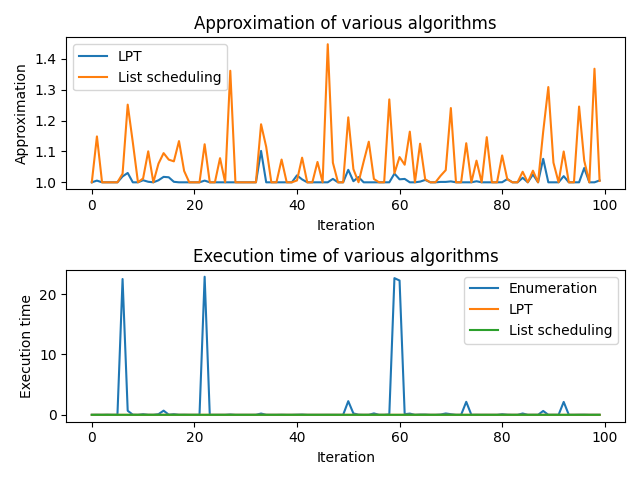
\includegraphics[scale = 0.7]{img/myplot.png}
\end{center}

Как видно из первого графика, оценка сверху на коэффициент приближения для обоих алгоритмов не нарушается. Более того, для сгенерированных входных данных алгоритмы $\sf{LPT}$ и $\sf{List}$ $\sf{scheduling}$ дают приближение не хуже $\frac{11}{10}$ и $\frac{3}{2}$ соответственно.

\begin{table}[h!]
\centering
 \caption{Итоговая таблица с замерами}
 \begin{tabular}{||c c c c||} 
 \hline
  & Enumeration & LPT & List scheduling \\ [0.5ex] 
 \hline\hline
 Average approximation coefficient & 1.000 & 1.010 & 1.045 \\ 
 Average execution time, sec. & $95901.678 \cdot 10^{-5}$ & $3.003 \cdot 10^{-5}$ & $4.004 \cdot 10^{-5}$ \\ [1ex]
 \hline
 \end{tabular}
\end{table}
